\documentclass[11pt]{article}
\usepackage[final]{acl}
\usepackage{times}
\usepackage{latexsym}
\usepackage[T1]{fontenc}
\usepackage[utf8]{inputenc}
\usepackage{microtype}
\IfFileExists{inconsolata.sty}{\usepackage{inconsolata}}{}
\usepackage{graphicx}
\usepackage{booktabs}
\usepackage{adjustbox}
\usepackage{amsmath}
\usepackage{xcolor}
\usepackage{tikz}
\usetikzlibrary{positioning,arrows.meta}
\usepackage{tcolorbox}
\usepackage{enumitem}
\setlist{nosep,leftmargin=*}

% numbers produced by src/analysis.py (results/tables/numbers.tex); \V{key} prints one
\newcommand{\nmdef}[2]{\expandafter\def\csname num@#1\endcsname{#2}}
\newcommand{\V}[1]{\ifcsname num@#1\endcsname\csname num@#1\endcsname\else\textcolor{red}{??\detokenize{#1}}\fi}
\InputIfFileExists{tables/numbers.tex}{}{}
\graphicspath{{figures/}}
\newcommand{\tabinput}[1]{\InputIfFileExists{tables/#1.tex}{}{\textcolor{red}{[\detokenize{#1} pending]}}}
% a one-column table: tighter column gaps, and shrunk only if still wider than the column
\newcommand{\fittab}[1]{{\setlength{\tabcolsep}{3.5pt}\adjustbox{max width=\columnwidth}{\tabinput{#1}}}}
\newcommand{\code}[1]{\texttt{\small #1}}

\title{Replicating ``A Watermark for Large Language Models''}

\author{Rupak Pantha (60824670) \\
  COMP8240 Applications of Data Science, Macquarie University}

\begin{document}
\maketitle

\begin{abstract}
\citet{kirchenbauer2023watermark} hide a statistical signal in language-model output: the model is nudged towards a pseudo-random ``green'' part of the vocabulary, and anyone with the key can detect the text with a $z$-test. We replicate the paper with the authors' code, the paper's own models (OPT-1.3B generator, OPT-2.7B oracle, T5-Large attacker) and its own data (\V{rep.n} C4 RealNewsLike prompts). Over the paper's $\gamma\times\delta$ grid our true-positive rates match the paper's within sampling error in five of six settings (\V{rep.tpr4.g0.5.d2} vs.\ 0.984 at $\gamma{=}0.5,\delta{=}2$), no held-out human text is flagged, and the T5 span attack degrades detection as reported. We also isolate a hardware dependence in the released code: text watermarked on the CPU scores at chance when detected on a GPU. We then build a \V{md.n}-prompt dataset from ten sources, nine of which the paper never used, each paired with a real human continuation: Wikipedia, CC-News, Project Gutenberg, IMDb, Reddit, Amazon reviews, Stack Exchange, ACL ethics statements and Python code. At $\delta{=}2$, \V{md.allnew.tpr_d2} of watermarked texts are detected. The raw $z$-score flags degenerate repetitive outputs and human-written code, but counting repeated bigrams once removes every false positive (0 of \V{md.all.nneg} human and \V{md.all.nneg} unwatermarked texts). Watermark strength follows the generator's spike entropy (Spearman $\rho=\V{md.rho.dedup}$), so code is the weak spot. A modern generator, Qwen2.5-1.5B, on the same prompts gives the same picture with far fewer false positives on code. An LLM judge shows that the paper's perplexity metric favours repetitive model text over human writing and that a watermark of $\delta\le2$ costs little quality; blind human ratings confirm both findings, although the judge agrees with them only weakly on single texts.
\end{abstract}

%=====================================================================
\section{The Paper and Why It Was Chosen}
\label{sec:paper}

\paragraph{Problem and method.}
Fluent machine-generated text can no longer be told apart from human writing by reading it, and regulation now requires it to be labelled: Article~50 of the EU AI Act asks providers to mark AI-generated content in a machine-readable, detectable way \citep{euaiact2024}. \citet{kirchenbauer2023watermark} propose a watermark that is applied while the text is generated, needs no retraining, and can be detected without the model. Before each token $s^{(t)}$ is sampled, the previous token $s^{(t-1)}$ seeds a pseudo-random generator that splits the vocabulary into a \emph{green list} of size $\gamma|V|$ and a red list. A constant $\delta$ is added to the logits of green tokens (a ``soft'' watermark), so green tokens become more likely without forbidding red ones. A detector that knows the key recomputes each green list and counts the green tokens $|s|_G$ among $T$ scored tokens. Under the null hypothesis that the text was written without knowledge of the lists, $|s|_G$ is binomial with mean $\gamma T$, giving
\begin{equation}
z=\frac{|s|_G-\gamma T}{\sqrt{T\gamma(1-\gamma)}} .
\label{eq:z}
\end{equation}
Text with $z>4$ (one-sided $p<3.2\times10^{-5}$) is declared watermarked. The paper also bounds the expected number of green tokens through the \emph{spike entropy} of the model's next-token distributions: when the model is nearly certain of the next token, the bias cannot change it, so low-entropy text carries a weaker watermark.

\paragraph{How the paper evaluated it.}
The authors watermark OPT-1.3B \citep{zhang2022opt} completions of $\sim$500 prompts from C4 RealNewsLike \citep{raffel2020t5}, with $T=200\pm5$ tokens, multinomial sampling at temperature 0.7 and 8-way beam search. \emph{Detectability} is measured by true- and false-positive rates (TPR, FPR) at $z>4$ and $z>5$ and by ROC/AUC (their Table~2 and Fig.~4). \emph{Text quality} is the perplexity (PPL) of each completion under a larger oracle model, OPT-2.7B, conditioned on the prompt (Fig.~2). \emph{Robustness} is tested with a T5-Large span-replacement attack that rewrites a fraction $\varepsilon$ of the tokens (Table~8, Fig.~6). The headline results are a TPR of 0.984 with \emph{zero} false positives at $\gamma{=}0.5,\delta{=}2$ (multinomial), a small PPL increase for moderate $\delta$, and a TPR that falls to 0.353 when an attacker replaces 30\% of the tokens, at a large cost in PPL.

\paragraph{Justification.}
The paper was chosen on four grounds. (i)~\emph{Venue}: ICML is ranked A* in ICORE2026, a rank held by 7.5\% of the 825 ranked venues \citep{icore2026}. (ii)~\emph{Recognition}: it received an ICML~2023 Outstanding Paper Award \citep{icml2023awards}. (iii)~\emph{Impact}: Semantic Scholar lists 1{,}148 citations on 1~November~2026, about eight times the next most-cited LLM-watermarking paper in the same search \citep{semanticscholar2026}, and the official repository has 697 stars and 91 forks. (iv)~\emph{Reproducibility and relevance}: the code is open (Apache-2.0), the models are public, and token-level watermarks such as SynthID-Text \citep{dathathri2024synthid} are now being deployed at scale in response to the EU AI Act.

%=====================================================================
\section{The Original Dataset}
\label{sec:origdata}

The paper's only text corpus is the \emph{RealNewsLike} subset of C4 \citep{raffel2020t5}.\footnote{\url{https://huggingface.co/datasets/allenai/c4}, config \code{realnewslike}; ODC-BY licence.} C4 is a cleaned Common Crawl scrape. RealNewsLike keeps the pages from the news domains of RealNews: 13.8M training and 13.9K validation documents (about 15\,GB) of English news prose. Each record is a JSON object with three fields (Figure~\ref{fig:c4}). The paper streams random documents, tokenises each one, and removes the final $T$ tokens as the \emph{human baseline} completion; the rest is the prompt. The other ``data'' in the evaluation are models: OPT-1.3B generates, OPT-2.7B scores perplexity, and T5-Large \citep{raffel2020t5} performs the attack.

\begin{figure}[t]
\begin{tcolorbox}[colback=gray!4,colframe=gray!50,boxrule=0.4pt,left=3pt,right=3pt,top=2pt,bottom=2pt,fontupper=\scriptsize\ttfamily\raggedright]
\{"url": "\V{c4.example.url}",\\
\phantom{\{}"timestamp": "\V{c4.example.ts}",\\
\phantom{\{}"text": "\V{c4.example.text}\ldots"\}
\end{tcolorbox}
\vspace{-2mm}
\caption{A C4 RealNewsLike record (text truncated). In the replication, the last 200 OPT tokens of \code{text} are held out as the human baseline and the rest, capped at 312 tokens, is the prompt.}
\label{fig:c4}
\end{figure}

%=====================================================================
\section{Replication of the Original Work}
\label{sec:rep}

\subsection{Environment and code}
Watermarking and detection use the authors' \code{WatermarkLogitsProcessor} and \code{WatermarkDetector} from \code{extended\_watermark\_processor.py} \citep{kirchenbauer2023code}, pinned to commit \code{8292251}. Their \code{simple\_1} seeding is the paper's LeftHash scheme ($h{=}1$). We added only the glue the paper's description specifies: prompt construction, a matched generation loop, the T5 attack, oracle perplexity and analysis. The authors' experiment launcher targets a GPU cluster, so we reused their library code rather than the launcher. A pilot of the whole study ran on a laptop CPU with OPT-350M. The final run used the paper's models on a single GPU in a Kaggle notebook (Python \V{env.python}, PyTorch \V{env.torch}, Transformers \V{env.transformers}, Datasets \V{env.datasets}) and took about nine hours. One self-contained notebook, which carries the code and resumes after interruptions, reproduces every number; code, data, results and this report are on GitHub.\footnote{\url{https://github.com/RupakO4/llm-watermark-replication}} To use the GPU efficiently, one batched \code{generate()} call produces the unwatermarked and all watermarked continuations of several prompts at once. Each row's green list is still computed by the authors' processor.

\subsection{Settings and remaining deviations}
We follow the paper's protocol (Sec.~\ref{sec:origdata}) on \V{rep.n} random C4 documents, the paper's sample size. For each prompt we sample one unwatermarked continuation and one watermarked continuation for every $(\gamma,\delta)\in\{0.25,0.5\}\times\{1,2,5\}$ from the same random stream. We use multinomial sampling at temperature 0.7 with no top-$k$/top-$p$ truncation, and $T=200$. Unwatermarked and human texts are scored under each $\gamma$, so every row of the paper's Table~2 has its own FPR. Four deviations remain: \textbf{(1)}~documents are truncated to 512 tokens (median prompt \V{rep.promptmed} tokens); \textbf{(2)}~EOS is suppressed until exactly $T$ tokens are generated, instead of discarding outputs outside $200\pm5$; \textbf{(3)}~the attack replaces a fraction $\varepsilon$ of \emph{words}, not tokens, on 200 of the \V{rep.n} texts; \textbf{(4)}~we did not run beam-search decoding of the watermarked model.

\subsection{A hardware dependence in the released code}
\label{sec:device}
Our first run (project update) detected watermarked text at chance level. The cause is that both the processor and the detector draw each green list with \code{torch.randperm} from a \code{torch.Generator} created on the \emph{model's} device. The same seed gives different permutations on CPU, Apple MPS and CUDA, so a detector on another device checks the wrong lists. We therefore draw every green list on the CPU, also when the model runs on the GPU. To confirm the effect, we re-scored \V{dev.n} watermarked replication texts ($\gamma{=}0.5,\delta{=}2$) with detectors built on each device. On CPU the mean $z$ is \V{dev.cpu.z} (\V{dev.cpu.det}/\V{dev.n} detected); on CUDA it is \V{dev.cuda.z} (\V{dev.cuda.det}/\V{dev.n}), as it was on MPS in our laptop pilot (0.01, 0/50). The ``secret key'' is therefore not just the hash seed but also the hardware random number generator, which matters for anyone deploying the scheme.

\subsection{Results}
\begin{table*}[t]
\centering\small
\tabinput{rep_grid}
\caption{Replication of Table~2 of \citet{kirchenbauer2023watermark} (OPT-1.3B, multinomial sampling, $T{=}200$) on \V{rep.n} C4 prompts. FPR is measured on the matched unwatermarked continuations and on the held-out human text, scored under the same $\gamma$; the paper reports FPR $=0$ for every row. 95\% Wilson intervals are shown for our TPR at $z>4$. PPL is the mean oracle (OPT-2.7B) perplexity.}
\label{tab:rep}
\end{table*}

\paragraph{Detection (Table~\ref{tab:rep}).}
Detection replicates closely. At the paper's headline setting ($\gamma{=}0.5,\delta{=}2$) we detect \V{rep.tpr4.g0.5.d2} of the watermarked texts, against 0.984 in the paper; at $\gamma{=}0.25$ we detect \V{rep.tpr4.g0.25.d2}, against 0.994. The paper's value lies inside our 95\% interval in four of the six settings and 0.001 above it at $\gamma{=}0.25,\delta{=}2$ (a difference of four texts). The exception is the weakest setting, $\gamma{=}0.5,\delta{=}1$, where we detect \V{rep.tpr4.g0.5.d1} against 0.767. No held-out human continuation exceeded $z{=}4$ under either $\gamma$. Two unwatermarked continuations did, both at $\gamma{=}0.25$ ($z$ of 4.90 and 5.23). Both are rambling, repetitive news pastiche, and counting each repeated bigram only once, as the paper recommends (its Sec.~4.1), lowers them to 0.79 and 1.84. Under that rule the $\delta{=}2$ TPR is still \V{rep.tpr4_dedup.g0.5.d2}.

\paragraph{Quality trade-off (Figure~\ref{fig:tradeoff}).}
The quality cost reproduces in direction and size. Unwatermarked OPT-1.3B text has a mean oracle PPL of \V{rep.ppl.unwatermarked}. The watermark raises it to \V{rep.ppl.g0.5.d2} at $\gamma{=}0.5,\delta{=}2$ and to \V{rep.ppl.g0.25.d5} at the strongest setting, while the mean $z$ climbs from \V{rep.z.g0.5.d1} to \V{rep.z.g0.25.d5}. As in the paper's Fig.~2, a smaller green list ($\gamma{=}0.25$) buys a stronger watermark at about the same PPL. Real human continuations score a PPL of \V{rep.ppl.human}, worse than all but the strongest watermark: the oracle prefers the model's predictable text to human prose, a first hint that PPL is a weak proxy for quality (Sec.~\ref{sec:judge}).

\begin{figure}[t]
\centering
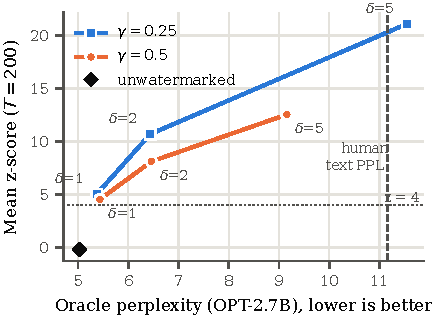
\includegraphics[width=\columnwidth]{rep_tradeoff.pdf}
\vspace{-6mm}
\caption{Watermark strength vs.\ text quality on C4, our analogue of the paper's Fig.~2 (left). Each point is one $(\gamma,\delta)$ setting averaged over \V{rep.n} prompts.}
\label{fig:tradeoff}
\end{figure}

\paragraph{Attack (Table~\ref{tab:t5}).}
We attacked 200 of the $\gamma{=}0.5,\delta{=}2$ texts with the paper's T5-Large span attack (50-way beam search, $k{=}20$ candidates). Detection degrades as in the paper: TPR \V{rep.t5.tpr4.e0.1} at $\varepsilon{=}0.1$ (paper 0.819), \V{rep.t5.tpr4.e0.3} at 0.3 (paper 0.353), \V{rep.t5.tpr4.e0.5} at 0.5 (0.094) and \V{rep.t5.tpr4.e0.7} at 0.7 (0.039). When repeated bigrams are counted once, the TPR is \V{rep.t5.tpr4_dedup.e0.3} at $\varepsilon{=}0.3$ and \V{rep.t5.tpr4_dedup.e0.5} at 0.5. From $\varepsilon{=}0.3$ on, the paper's values therefore lie between our two scoring rules: repeated phrases that the attack misses keep scoring green under the raw rule. The attack is not free for the attacker. Oracle PPL nearly doubles, from \V{rep.t5.ppl.e0} to \V{rep.t5.ppl.e0.5} at $\varepsilon{=}0.5$, and the AUC stays at \V{rep.t5.auc.e0.5}, so attacked text is still ranked above unwatermarked text even below the $z{=}4$ threshold, as in the paper's Fig.~6.

\begin{table}[t]
\centering\small
\fittab{rep_t5}
\caption{T5-Large span-replacement attack (50 beams) on 200 $\gamma{=}0.5,\delta{=}2$ texts (paper Table~8, multinomial). $\varepsilon$ is the replacement budget and ``real.'' the fraction of words actually replaced. AUC is against the unwatermarked texts.}
\label{tab:t5}
\end{table}

\paragraph{Why the numbers differ, and where the method fails.}
With \V{rep.n} prompts, a TPR difference of 0.02 is ten texts, within sampling error. The one significant gap, $\gamma{=}0.5,\delta{=}1$, is the setting most sensitive to entropy: the mean spike entropy of OPT-1.3B in our contexts is \V{gap.g0.5.d1.spike_mean}, below the 0.807 the paper reports for the same model, so each token carries less watermark. We tested this with data we already had (Appendix~\ref{app:gap}). Entropy matters: TPR rises from \V{gap.g0.5.d1.tpr_low} in the least to \V{gap.g0.5.d1.tpr_high} in the most entropic third of prompts, and a logistic fit predicts \V{gap.g0.5.d1.pred_paper} at the paper's mean entropy (paper: 0.767). Forcing exactly 200 tokens is \emph{not} the cause: tokens 101--200 are as green as tokens 1--100 (\V{gap.g0.5.d1.green2} vs.\ \V{gap.g0.5.d1.green1}). Truncating documents to 512 tokens may contribute: our longest-context prompts are detected at \V{gap.g0.5.d1.tpr_cap} and shorter ones at \V{gap.g0.5.d1.tpr_short} ($p=\V{gap.g0.5.d1.cap_p}$). The same fit overshoots the paper at $\gamma{=}0.25$ (\V{gap.g0.25.d1.pred_paper} vs.\ 0.729), so entropy is not the whole story. Our six misses at $\gamma{=}0.5,\delta{=}2$ show the failure mode the paper describes for low-entropy text (its Table~4): sports fixture lists, newsletter boilerplate (``\ldots\ Business Insider Email'') and loops.

%=====================================================================
\section{Construction of New Data}
\label{sec:newdata}

\paragraph{Design.}
Our earlier dataset (project update) used prompts drafted with an AI assistant. They had no provenance and no human reference, and the marker asked for more detail on collection and preprocessing and for tests on more kinds of text. The final dataset therefore starts every prompt from a \emph{real document} with a citable source, licence and row index. The next 150 tokens of that same document are held out as a \emph{human continuation}, which serves as the negative control, exactly as the paper uses C4. We took 100 documents from each of ten sources (Table~\ref{tab:sources}): C4 itself, kept as an anchor, plus nine registers the paper never tested. They cover encyclopedic, news, literary, opinion, conversational, consumer, technical, scientific and source-code text: Wikipedia \citep{wikipedia2023}, CC-News \citep{hamborg2017newsplease}, Project Gutenberg \citep{gutenberg}, IMDb reviews \citep{maas2011imdb}, Reddit posts \citep{volske2017tldr}, Amazon reviews \citep{hou2024amazon}, Stack Exchange answers \citep{h4stackexchange}, ACL ethics statements \citep{karamolegkou2025ethicon} and the Python standard library \citep{python}. Two of them come from the proposal's plan (Reddit, Amazon), Stack Exchange replaces AnswerSumm (the same source, but distributed as parquet), and the ACL ethics statements come from the EthiCon corpus recommended in the unit \citep{karamolegkou2025ethicon}.

\begin{table*}[t]
\centering\scriptsize
\tabinput{data_sources}
\caption{Sources of the new data, 100 prompts each. ``Scanned'' counts streamed documents; the rejection reasons are the filters of Sec.~\ref{sec:newdata}. ``Released'' says whether the source text itself is redistributed in our repository (otherwise only identifiers, hashes and our model outputs are).}
\label{tab:sources}
\end{table*}

\paragraph{Collection and preprocessing.}
\code{build\_prompts.py} streams each corpus with a seeded shuffle (seed 42, buffer 2{,}000), so the sample can be rebuilt exactly and nothing is downloaded in full. It processes each document as follows:
\begin{enumerate}
\item \emph{Normalise}: Unicode NFKC and consistent newlines.
\item \emph{Strip markup per source}: HTML tags, entities and \code{<pre>} code blocks from Stack Exchange answers (\V{data.stackexchange.code_blocks_removed} code blocks removed); \code{<br />} tags from IMDb and Amazon; the licence header and the first 5{,}000 characters (title page and contents) from Gutenberg books; hyphenated line breaks and hard wraps from the PDF-extracted ethics statements (\V{data.acl_ethics.hyphenation_joins} joins; Figure~\ref{fig:snippet}a).
\item \emph{Remove personal data}: replace e-mail addresses, URLs, phone numbers and Reddit usernames with placeholders (\V{data.all.pii} replacements, most of them digit runs in Gutenberg books). Reject documents dominated by them (link farms, contact lists).
\item \emph{Filter}: reject texts under 600 characters, with fewer than 55\% letters, in a non-Latin script, or dominated by tables or wiki markup. For informal sources, reject explicit or abusive posts using a short keyword list and NSFW subreddit names.
\item \emph{Cut the span}: start at the first sentence-like boundary. The prompt is the next 50 OPT tokens and the human continuation the following 150; shorter documents are rejected.
\item \emph{De-duplicate} on a hash of the prompt, and record source, split, revision, row index, metadata, licence and SHA-256.
\end{enumerate}
Every rejection is counted by reason (Table~\ref{tab:sources}). Amazon reviews were the hardest to fill: \V{data.amazon.scanned} were read to keep 100, and almost all of the rejected ones were too short. The safety filters removed 42 IMDb and Reddit posts. Eighteen Gutenberg books tripped the contact-detail filter; in public-domain books this most likely means tables of numbers, but we kept the filter conservative. A fixed 50-token prompt keeps the text domain as the only thing that changes between sources.

\paragraph{Generated data.}
Each of the \V{md.n} prompts is continued by OPT-1.3B with the replication's sampler. This gives one unwatermarked and three watermarked continuations at $\gamma{=}0.5$, $\delta\in\{1,2,5\}$. The $\delta{=}2$ text is then edited by eight automatic attacks: whitespace normalisation, deletion and random substitution of 10/30/50\% of the words, and a dictionary synonym swap. For 10 prompts per source we also run the T5 span attack at $\varepsilon\in\{0.1,0.3,0.5\}$. Together with the human continuations this gives \V{md.ntexts} labelled texts. To test whether the findings depend on the generator, the same prompts are also continued by a modern model, Qwen2.5-1.5B \citep{qwen2025qwen25}, re-tokenised for its vocabulary (5{,}000 more texts). Each row records the generation settings, token ids, green fraction, $z$ (raw, repeated-bigram-ignored, and at $T{=}25$--150), oracle PPL, generator entropy and judge scores (Figure~\ref{fig:snippet}b).

\begin{figure}[t]
\begin{tcolorbox}[colback=gray!4,colframe=gray!50,boxrule=0.4pt,left=3pt,right=3pt,top=2pt,bottom=2pt,fontupper=\scriptsize]
\textbf{(a) EthiCon statement, raw vs.\ cleaned}\\
\emph{Raw:} \V{snip.acl.raw}\\[1pt]
\emph{Cleaned:} \V{snip.acl.clean}\\[3pt]
\textbf{(b) One prompt and three continuations (\V{snip.row.id})}\\
\emph{Prompt:} \V{snip.row.prompt}\\
\emph{Human:} \V{snip.row.human}\\
\emph{Unwatermarked} ($z{=}\V{snip.row.zu}$): \V{snip.row.unwm}\\
\emph{Watermarked} $\delta{=}2$ ($z{=}\V{snip.row.zw}$): \V{snip.row.wm}
\end{tcolorbox}
\vspace{-2mm}
\caption{Snippets of the new data (continuations truncated).}
\label{fig:snippet}
\end{figure}

\paragraph{Human annotation.}
Detection labels come from the generation process, so they need no annotation. Text \emph{quality}, however, does, and we used an LLM judge for it (Sec.~\ref{sec:judge}). To check that judge, we drew 60 continuations from the pilot run that were balanced over condition (human, unwatermarked, $\delta{=}2$, $\delta{=}5$) and source, used each prompt at most once, and hid the condition. Two annotators rated them independently in a stand-alone browser tool (\code{annotate.html}) on the same 1--5 rubric the judge receives (Appendix~\ref{app:judge}): the author and a second annotator not involved in the project, who did not see the author's ratings. Both the pilot's judge and the final judge rated the same texts. The second annotator flagged one continuation as sexually explicit; it was removed (Sec.~\ref{sec:ethics}), leaving \V{hh.n} items. Agreement is measured with quadratically weighted Cohen's $\kappa$ \citep{cohen1968weighted}, which suits ordinal scales.

%=====================================================================
\section{Results on the New Data}
\label{sec:results}

\begin{table*}[t]
\centering\scriptsize
\tabinput{md_sources}
\caption{Results on the new data (OPT-1.3B, $\gamma{=}0.5$, $T{=}150$, 100 prompts per source, sorted as in Fig.~\ref{fig:sources}). $S$: mean spike entropy of the generator along the $\delta{=}2$ texts. TPR at $z>4$ for each $\delta$; for $\delta{=}2$ also the mean $z$, the TPR when repeated bigrams are counted once (``dedup'', paper Sec.~4.1) and after only 50 tokens. FP: false positives among 100 human and 100 unwatermarked texts, raw/dedup. Judge: mean expected LLM-judge rating.}
\label{tab:md}
\end{table*}

\paragraph{Detection generalises (Table~\ref{tab:md}).}
The watermark is detected on the new sources as reliably as on C4. At $\delta{=}2$, \V{md.allnew.tpr_d2} of the 900 watermarked texts from the nine new sources exceed $z{=}4$ (C4 under the same protocol: \V{md.c4.tpr_d2}), and every $\delta{=}5$ text is detected. The weak $\delta{=}1$ setting varies most by source, from \V{md.cc_news.tpr_d1} on CC-News and \V{md.wikipedia.tpr_d1} on Wikipedia to \V{md.reddit.tpr_d1} on Reddit. Informal and opinionated writing carries the mark best; encyclopedic and news text, which includes the paper's own domain, is the hardest. Under raw scoring, 7 of the 1{,}800 human and unwatermarked prose texts reach $z{=}4$. Six are degenerate model outputs (``AHAHAHA\ldots'', runs of blank space, repeated lines) and one is a human ethics statement at $z{=}4.08$; counting repeated bigrams once lowers all seven below 3.4. Python code is the real exception. There, \V{md.python_code.fp_human} of 100 human-written continuations and \V{md.python_code.fp_unwm} of 100 unwatermarked ones are falsely flagged, with $z$ up to \V{md.python_code.z_unwm_max}. Code repeats bigrams such as indentation runs and \code{self.} far more often than prose, which breaks the independence the $z$-test assumes. Counting repeated bigrams once removes every false positive, but it also removes most of the signal. Only \V{md.python_code.tpr_d2_dedup} of watermarked code is then detected, because a 150-token code continuation contains only \V{md.python_code.uniq_d2} distinct bigrams on average (prose: \V{md.allnew.uniq_d2}). On code from this model the scheme is either unsafe or nearly blind, depending on the scoring rule.

\paragraph{Watermark strength follows entropy (Figure~\ref{fig:sources}).}
The raw $z$-score barely tracks the generator's entropy (Spearman $\rho=\V{md.rho}$ over \V{md.rho.n} texts), because repetition inflates $z$ precisely in low-entropy text. Once repeated bigrams are counted only once, the relationship the paper derives in its Theorem~4.2 appears clearly: $\rho=\V{md.rho.dedup}$ between mean spike entropy and $z$ (Fig.~\ref{fig:sources}b). Code has by far the lowest spike entropy (\V{md.python_code.spike}, against \V{md.allnew.spike} overall) and the weakest real signal. Among the prose sources, Gutenberg loses most when repeats are removed, because its $\delta{=}2$ continuations often loop (distinct-2 of \V{md.gutenberg.distinct2_d2}, against \V{md.gutenberg.distinct2_human} for the human text).

\begin{figure*}[t]
\centering
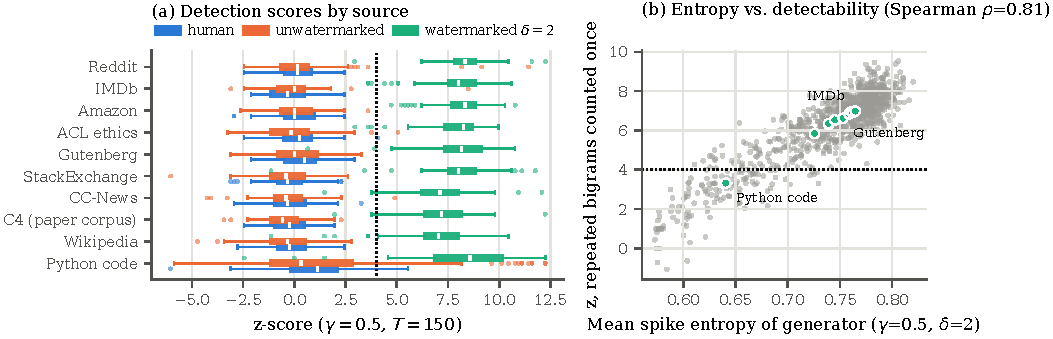
\includegraphics[width=\textwidth]{sources.pdf}
\vspace{-6mm}
\caption{(a) $z$-scores of human, unwatermarked and watermarked ($\delta{=}2$) text for each source. The dotted line is the detection threshold $z{=}4$. (b) Each grey point is one watermarked text; green dots are source means. Watermark strength rises with the generator's spike entropy, as the paper's theory predicts.}
\label{fig:sources}
\end{figure*}

\paragraph{Length and robustness (Figures~\ref{fig:length}, \ref{fig:robust}).}
Short texts need a stronger watermark. At $\delta{=}2$, \V{md.len.d2.T50} of the texts are detected after 50 tokens, \V{md.len.d2.T100} after 100 and \V{md.len.d2.T150} after 150; at $\delta{=}5$, \V{md.len.d5.T25} are already detected after 25 tokens (Fig.~\ref{fig:length}). Edits weaken detection on the new data in the same way as on C4 (Fig.~\ref{fig:robust}). Substituting 10\% of the words barely matters (TPR \V{rob.md.random_substitute_0.1}), 30\% lowers TPR to \V{rob.md.random_substitute_0.3}, and 50\% to \V{rob.md.random_substitute_0.5}. Deleting words does less damage than substituting them, because each deletion changes only one green list. Dictionary synonyms leave detection intact (\V{rob.md.synonym}); normalising whitespace costs a few points (\V{rob.md.whitespace}) because some continuations contain runs of blank-space tokens. The T5 span attack matches random substitution at 30\% of words replaced (TPR \V{rob.md.t5_span_0.3}) but is weaker at 50\% (\V{rob.md.t5_span_0.5}; Appendix Table~\ref{tab:robust}); counting repeats once lowers these to \V{rob.md.t5_span_0.3.dedup} and \V{rob.md.t5_span_0.5.dedup}. The texts still detected after a 50\% attack are the repetitive ones (55\% of their bigrams are distinct, against 72\% for all attacked texts), whose repeated phrases inflate the raw score but carry little independent evidence.

\begin{figure}[t]
\centering
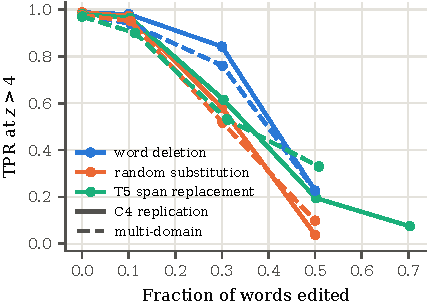
\includegraphics[width=\columnwidth]{robustness.pdf}
\vspace{-6mm}
\caption{TPR ($z>4$) of $\gamma{=}0.5,\delta{=}2$ text against the fraction of words edited, for three attacks, on the C4 replication (solid) and the new data (dashed).}
\label{fig:robust}
\end{figure}

\begin{figure}[t]
\centering
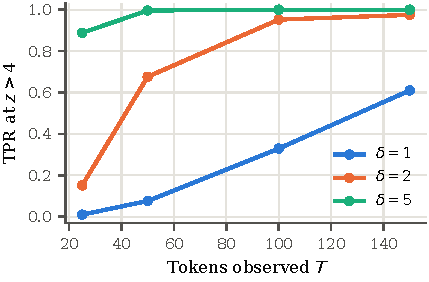
\includegraphics[width=\columnwidth]{length.pdf}
\vspace{-6mm}
\caption{TPR ($z>4$) on the new data when only the first $T$ generated tokens are scored.}
\label{fig:length}
\end{figure}

\paragraph{A modern generator (Table~\ref{tab:modern}).}
The paper's model is from 2022. Repeating the new-data study with Qwen2.5-1.5B (2024) on the same documents gives the same overall picture: \V{mod.allnew.tpr_d2} of $\delta{=}2$ texts from the nine new sources are detected (OPT-1.3B: \V{md.allnew.tpr_d2}), every $\delta{=}5$ text is detected, and spike entropy again predicts the repeat-discounted $z$ ($\rho=\V{mod.rho.dedup}$). Two things change. First, Qwen produces far fewer degenerate outputs, so raw scoring flags only \V{mod.all.fp_human} human and \V{mod.all.fp_unwm} unwatermarked texts out of \V{mod.all.n_neg} each (OPT-1.3B: \V{md.all.fp_human} and \V{md.all.fp_unwm}), and none with repeats discounted. On code this matters most. Qwen's code repeats less (\V{mod.python_code.uniq_d2} distinct bigrams per continuation against \V{md.python_code.uniq_d2}), so only two code texts are falsely flagged, and \V{mod.python_code.tpr_d2_dedup} of watermarked code survives deduplication (OPT-1.3B: \V{md.python_code.tpr_d2_dedup}). Second, the weak spots move. For Qwen, encyclopedic text joins code at the bottom: Wikipedia has $S{=}\V{mod.wikipedia.spike}$ and a $\delta{=}2$ TPR of \V{mod.wikipedia.tpr_d2}, code $S{=}\V{mod.python_code.spike}$ and \V{mod.python_code.tpr_d2}. A more confident model writes text that carries less watermark, as Theorem~4.2 predicts, so the right $\delta$ depends on both the model and the domain. By the judge, Qwen writes better text (unwatermarked \V{mod.allnew.judge_unwm} vs.\ \V{md.allnew.judge_unwm}). $\delta{=}2$ costs it more (down to \V{mod.allnew.judge_d2}, against \V{md.allnew.judge_d2} for OPT-1.3B), but its watermarked text is still rated above OPT's unwatermarked text.

\begin{table*}[t]
\centering\scriptsize
\tabinput{modern_compare}
\caption{The same \V{md.n} new-data prompts continued by the paper's model and by a modern one ($\gamma{=}0.5$, $\delta{=}2$, $T{=}150$). $S$: spike entropy. FP: false positives among each source's human and unwatermarked texts, raw/dedup. Judge: mean expected rating of the $\delta{=}2$ texts.}
\label{tab:modern}
\end{table*}

\paragraph{Quality: perplexity vs.\ an LLM judge.}
\label{sec:judge}
The paper measures quality only with oracle PPL. We added an LLM-as-judge \citep{zheng2023judging}: Qwen2.5-3B-Instruct \citep{qwen2025qwen25}, run locally so that the evaluation is reproducible and free. It sees a shortened prompt and one continuation, never the condition, and rates the continuation from 1 to 5 for fluency, coherence and repetition (Appendix~\ref{app:judge}). Rather than sample an answer, we read the judge's probabilities for the tokens ``1''--``5'' and use the expected rating. The two measures agree that the watermark costs quality and that the cost grows with $\delta$ (Table~\ref{tab:judge}). On the new data, median PPL rises from \V{judge.md.unwatermarked.ppl} for unwatermarked text to \V{judge.md.wm_d2.ppl} at $\delta{=}2$ and \V{judge.md.wm_d5.ppl} at $\delta{=}5$, and the judge's mean rating falls from \V{judge.md.unwatermarked} to \V{judge.md.wm_d2} and \V{judge.md.wm_d5}. On C4 the rating falls from \V{judge.rep.unwatermarked} to \V{judge.rep.wm_d2} at $\delta{=}2$, inside overlapping 95\% bootstrap intervals, and to \V{judge.rep.wm_d5} at $\delta{=}5$, with an interval (\V{judge.rep.wm_d5.lo}--\V{judge.rep.wm_d5.hi}) entirely below the unwatermarked one (\V{judge.rep.unwatermarked.lo}--\V{judge.rep.unwatermarked.hi}). The measures disagree about human text. The oracle gives human continuations the \emph{worst} PPL (\V{judge.md.human.ppl}), while the judge rates them clearly \emph{best} (\V{judge.md.human}, interval \V{judge.md.human.lo}--\V{judge.md.human.hi}). Across all texts, low PPL goes with \emph{low} ratings (Spearman $\rho=\V{judge.md.rho.ppl}$) and with repetition ($\rho=\V{judge.md.rho.ppldist}$ between PPL and distinct-2). The oracle rewards the loops that language models and strong watermarks produce, so the judge measures something PPL cannot. By its account, $\delta{\le}2$ costs about a tenth of a rating point, and $\delta{=}5$ two to five times as much.

\begin{table}[t]
\centering\small
\fittab{judge_quality}
\caption{Quality by condition (OPT-1.3B, $\gamma{=}0.5$). PPL: median OPT-2.7B perplexity. dist-2: share of distinct word bigrams (lower = more repetitive). Judge: mean expected Qwen2.5-3B rating (1--5).}
\label{tab:judge}
\end{table}

\paragraph{Is the judge trustworthy?}
The two annotators agree moderately with each other: quadratic $\kappa=\V{hh.kq}$ (linear \V{hh.kl}), \V{hh.within1} of ratings within one point, Spearman $\rho=\V{hh.rho}$. This human--human agreement is the ceiling a judge can be held to. The pilot's 1.5B judge reaches it, with $\kappa=\V{jc.j15.kq}$ against the author and \V{hh.kq_j15_r2} against the second annotator. The final 3B judge ranks the texts about as well (Spearman $\rho=\V{jc.j3.rho}$ with the author, against \V{jc.j15.rho}), but on a much harsher scale: its mean rating is \V{jc.j3.mean} against the author's \V{jc.human.mean}, and it gives the lowest rating to \V{jc.j3.ones} texts, mostly code and Wikipedia. Its exact agreement is therefore weak ($\kappa=\V{jc.j3.kq}$ and \V{hh.kq_j3_r2}). A larger judge was not a better-calibrated one. The human ratings nevertheless confirm, independently, the two conclusions drawn from the judge on the full data. First, averaged over both annotators, quality falls with $\delta$: human text \V{hh.avg.human}, unwatermarked \V{hh.avg.unwatermarked}, $\delta{=}2$ \V{hh.avg.watermarked_d2}, $\delta{=}5$ \V{hh.avg.watermarked_d5}. With about 15 items per condition, the gap between human text and $\delta{=}5$ is significant for the author (Mann--Whitney $p=\V{jc.mw.human_d5}$) and borderline for the average ($p=\V{hh.mw_human_d5}$). Second, perplexity misranks quality: the average human rating rises with oracle PPL ($\rho=\V{hh.rho_ppl_avg}$, $p=\V{hh.p_ppl_avg}$). We therefore use the judge only for averages over hundreds of texts per condition, where its ordering (human $>$ unwatermarked $>\delta{=}1>\delta{=}2>\delta{=}5$) is the same on both datasets, and never to score a single text.

\paragraph{How this relates to the replication.}
This evaluation differs from the replication in three ways: 150 instead of 200 generated tokens, fixed 50-token prompts instead of long news prefixes, and $\gamma{=}0.5$ only. Running C4 under the new protocol separates the effect of these choices from the effect of the domain. At $\delta{=}2$ the C4 TPR is \V{md.c4.tpr_d2} (replication: \V{rep.tpr4.g0.5.d2}). At $\delta{=}1$ it drops to \V{md.c4.tpr_d1} (replication: \V{rep.tpr4.g0.5.d1}), as expected with a quarter fewer tokens. Against that anchor, the new prose sources are within a few points of C4 (Wikipedia and CC-News slightly harder at $\delta{=}1$), and only code behaves differently. The paper's claims therefore hold for natural-language registers it never tested and for a newer model: near-certain detection at $\delta{=}2$, no false positives on human prose once repeats are discounted, and a gradual decline under edits. The caveat is that the false-positive guarantee needs the repeated-$n$-gram rule, and on repetitive code that rule removes much of the signal.

%=====================================================================
\section{Ethical Considerations}
\label{sec:ethics}

\paragraph{In the original work.}
The paper has no ethics or broader-impact statement, which is common: more than a third of ACL ethics statements identify no concern at all \citep{karamolegkou2025ethicon, benotti2022ethics}. Using EthiCon's most frequent concern labels (bias, misuse, privacy, misinformation), which map onto the risk areas of \citet{weidinger2021ethical}, we see four issues.
\begin{itemize}
\item \emph{Bias and false accusation.} The $z$-test bounds false positives only under the null hypothesis. Formulaic human writing (lists, templates, code) breaks the independence assumption, and detectors of AI text have penalised non-native writers \citep{liang2023detectors}. Under raw scoring our human controls produced \V{md.all.fp_human} false positives in \V{md.all.nneg}, five of them on code and one on an ethics statement; a deployment that could accuse a person needs the repeated-$n$-gram rule and far more evidence.
\item \emph{Misuse and spoofing.} Whoever holds the key can detect, and, by sampling green tokens, could also \emph{forge} watermarked text and attribute it to a model \citep{sadasivan2023detect}. Our attack results show that a determined user can remove the mark, so absence of a watermark proves nothing.
\item \emph{Privacy.} A key-holder can test any text a user wrote with model help, so detection is a form of surveillance and should be governed by policy.
\item \emph{Misinformation.} Watermarks help label synthetic content as required by \citet{euaiact2024}, but only for cooperating providers.
\end{itemize}

\paragraph{In our new data.}
We follow the principles of the \emph{Australian Code for the Responsible Conduct of Research} \citep{nhmrc2018code}, especially honesty, rigour, transparency, respect and recognition.
\begin{itemize}
\item \emph{Respect for people in the data.} Reddit, Amazon, IMDb and Stack Exchange texts are written by members of the public who did not consent to this use. Under the \emph{National Statement on Ethical Conduct in Human Research} \citep{nhmrc2023statement}, public availability does not imply consent, and posts that can be found again by verbatim search remain identifiable, so this use would not qualify for the exemption for negligible-risk research on non-identifiable data (para.~5.1.17). We judge the risk to be negligible in substance: no personal information is sought, explicit and abusive posts are filtered, usernames, e-mails, URLs and phone numbers are removed, and no author fields are kept. A publication using these rows should still go through ethics review.
\item \emph{Recognition and licences.} Each row carries its source and licence. The repository redistributes text only from openly licensed sources: CC BY-SA (Wikipedia, Stack Exchange), CC BY (ACL Anthology, Reddit dump), public domain (Gutenberg), ODC-BY (C4) and PSF (Python). CC-News articles and Amazon and IMDb reviews are released only as identifiers, hashes and our model outputs, and \code{build\_prompts.py} rebuilds them deterministically. The EthiCon repository states no licence, so we rely on the CC BY 4.0 licence of the ACL papers it quotes.
\item \emph{Course material.} The corpus built from our own lecture slides for the project update is copyrighted teaching material and was dropped from the released data.
\item \emph{Screening model output.} Filtering the prompts does not control what the model writes. We searched all 24{,}897 model-written texts (including edited and T5-attacked copies) for sexual terms and read every hit in context. Eighteen outputs (34 rows with their edited copies) were sexually explicit, described sexual assault graphically, or sexualised teenagers; the last came from a review of a school prom, whose continuations we removed for both models. We deleted their text from the raw and the released data and kept their scores, so all reported numbers still reproduce (\code{data/removed\_texts.csv}). One of them, which the second annotator flagged, had been in the annotation set and was excluded.
\item \emph{Annotation and AI use.} The human ratings come from the author and one volunteer second annotator, not from paid crowdworkers. Generative AI helped in correcting errors in code and proofread the report.\end{itemize}

%=====================================================================
\section{Conclusions and Reflections}
\label{sec:conc}
\paragraph{Replication.} Replication succeeded. With the authors' code, the paper's own models and the paper's sample size, we reproduced Table~2 within sampling error in five of six settings (TPR \V{rep.tpr4.g0.5.d2} vs.\ 0.984 at the headline setting, no false positives on human text), the strength--perplexity trade-off of Fig.~2, and the decline under T5 span replacement of Table~8. The weakest setting ($\gamma{=}0.5,\delta{=}1$) fell short, most likely because the generator's entropy is lower in our setting than in the paper's, plausibly because we truncate long documents (Appendix~\ref{app:gap}). The one real failure was in the released implementation, not the method: green lists depend on the hardware random number generator, so a text watermarked on one device is invisible to a detector on another.

\paragraph{Generalisation.} The approach generalises to every natural-language register we tried, from Reddit posts and Amazon reviews to Gutenberg fiction and ACL ethics statements, and to a newer model. Detection at $\delta{=}2$ stays near 0.98, and once repeated bigrams are counted once no human or unwatermarked text is flagged. Without that rule, degenerate model loops and human-written code produce false positives. Code is where the scheme is weakest: repetition breaks the $z$-test's guarantee, and once repeats are discounted too little entropy remains for a strong signal, as the paper's own theory predicts. Code-specific schemes that watermark only high-entropy tokens address exactly this case \citep{lee2024code}. Finally, an LLM judge and blind human ratings both showed that the paper's perplexity metric can mislead: it ranks repetitive model text above human writing.

\paragraph{Reflections.} (1)~\emph{Dataset design.} Our first constructed dataset, AI-drafted prompts for the project update, was the wrong design: it had no provenance and no human baseline. Starting every prompt from a real document with a held-out continuation made every result traceable and gave a real-text false-positive rate at no extra cost. (2)~\emph{Scale changed a conclusion.} Our pilot (OPT-350M, 300 new-data prompts) saw no false positive on prose; with \V{md.n} prompts and OPT-1.3B, raw scoring flagged seven. Rare failures need large samples, and the scoring rule belongs in every reported number. (3)~\emph{A bigger judge is not a better one.} Moving from a 1.5B to a 3B judge kept its ranking of texts but shifted its whole scale downwards, and weighted $\kappa$ with the human fell from \V{jc.j15.kq} to \V{jc.j3.kq}. The smaller judge agreed with each annotator as well as the two annotators agreed with each other ($\kappa=\V{hh.kq}$), so judges need to be calibrated against people, not chosen by size. (4)~\emph{Compute shaped the study.} Device-dependent randomness and a laptop that could not hold T5-Large cost more time than any analysis. Moving to a free cloud GPU, with green lists still drawn on the CPU, removed most deviations from the paper; a paraphrase attack \citep{kirchenbauer2024reliability} would be the next step.

\bibliography{references}

\appendix
\section{LLM-Judge Prompt}
\label{app:judge}
\begin{tcolorbox}[colback=gray!4,colframe=gray!50,boxrule=0.4pt,fontupper=\scriptsize\ttfamily]
\tabinput{judge_prompt}
\end{tcolorbox}
The judge's chat template is applied and the next-token probabilities of ``1''--``5'' are renormalised; we report $\sum_k k\,p(k)$. Human annotators saw the same rubric.

\section{Investigating the $\gamma{=}0.5,\delta{=}1$ Gap}
\label{app:gap}
\begin{table}[h]
\centering\small
\fittab{gap_table}
\caption{Testing explanations for the replication gap, on the \V{rep.n} C4 prompts. Entropy thirds split prompts by the generator's mean spike entropy $S$ (OPT-1.3B, measured along the unwatermarked continuation). ``green frac.'' is the share of green tokens among tokens 1--100 and 101--200. The last column is the TPR a logistic fit of detection on $S$ predicts at the paper's mean $S{=}0.807$ (paper's TPR in brackets).}
\label{tab:gap}
\end{table}
We tested the two protocol changes that could lower the watermark's strength at $\delta{=}1$ (Table~\ref{tab:gap}).

\emph{Forced length.} If suppressing EOS made the model pad its text with low-entropy filler after a natural ending, the second half of each text would carry less watermark. It does not: the green fraction of tokens 101--200 equals that of tokens 1--100 in every setting (Wilcoxon $p=\V{gap.g0.5.d1.green_p}$ at $\gamma{=}0.5,\delta{=}1$).

\emph{Entropy and context length.} Detection rises with the generator's spike entropy in all three settings (Spearman $\rho=\V{gap.g0.5.d1.rho}$ between $S$ and $z$ at $\gamma{=}0.5,\delta{=}1$, $p=\V{gap.g0.5.d1.rho_p}$). Our document cap of 512 tokens limits prompts to 312 tokens; \V{gap.g0.5.d1.n_cap} prompts hit this cap. Longer prompts give higher entropy ($\rho=\V{gap.g0.5.d1.rho_len}$), and capped prompts are detected more often (\V{gap.g0.5.d1.tpr_cap} vs.\ \V{gap.g0.5.d1.tpr_short}, Fisher $p=\V{gap.g0.5.d1.cap_p}$). The paper does not describe truncating documents, so its contexts were likely longer than ours, which would be consistent with its higher entropy.

\emph{What remains.} At the paper's mean entropy the fit predicts a TPR of \V{gap.g0.5.d1.pred_paper} at $\gamma{=}0.5$, close to the paper's 0.767, but \V{gap.g0.25.d1.pred_paper} at $\gamma{=}0.25$, above the paper's 0.729. Both predictions extrapolate to the top of our range (maximum $S$ = \V{gap.g0.5.d1.spike_max}), and the paper does not say how it averaged spike entropy, so lower entropy explains the direction of the $\gamma{=}0.5$ gap but not every difference.

\section{Additional Results}
\label{app:extra}
\begin{table}[h]
\centering\small
\fittab{robust_table}
\caption{Every edit attack at $\gamma{=}0.5,\delta{=}2$ (OPT-1.3B). ``edited'' is the realised fraction of words changed. TPR uses $z>4$.}
\label{tab:robust}
\end{table}
All per-text scores, the settings of every stage and the exact software environment are released with the code. The analysis script \code{src/analysis.py} regenerates every table, figure and number in this report from them.

\end{document}
